\documentclass[12pt,a4paper]{article}
\synctex=1
\usepackage[utf8]{inputenc}
\usepackage[margin=1cm]{geometry}
\usepackage{graphicx}
%\usepackage{verbatim}
\usepackage{amsmath}
\usepackage{amsfonts}
\usepackage{amssymb}
\usepackage{listings}
\usepackage{enumitem}
\usepackage{textcomp}
\usepackage{courier}
\usepackage{libertine}
\usepackage{pgfornament}
\usepackage{eso-pic}
\usepackage[hangul]{kotex}
\linespread{1.3}

\title{
	\centering
	\pgfornament[width=12cm,color=teal]{84}\\
	\vspace{1cm}
	\fontsize{50}{50} \selectfont {정보통신 수학 및 실습\\Homework}\\
		\pgfornament[width=12cm,color=teal]{88}\\
	\vfill}
\author{
	\LARGE
	\begin{tabular}{rl}
		\hline
		학번 : & 2016110056\\ 
		학과 : & 불교학부 \\
		이름 : & 박승원\\
		날짜 : & \today\\
		\hline
	\end{tabular}\vspace{2cm}
	\\
\includegraphics[width=0.5\textwidth]{logo.jpg}
	}
\date{}


\begin{document}
\maketitle
\pagenumbering{gobble}
\noindent
\lstset{language=matlab, columns=flexible, tabsize=4, frame=shadowbox, showstringspaces=false, breaklines=true, upquote=true, basicstyle=\normalsize}

\renewcommand{\thesubsubsection}{\alph{subsubsection})}
\renewcommand{\thesubsection}{\arabic{subsection}.}
\newpage

\section*{Chapter 8 Homework}
\subsection{If the outlet is a pipe that discharges to atmospheric pressure pa and provides a resistance, R, to flow that is proportional to the pressure difference across its ends, then find the outlet flow rate qmo and the differential equation of h(t).  Hint: qmo is (1/R)* (the pressure difference across its ends) } 
	
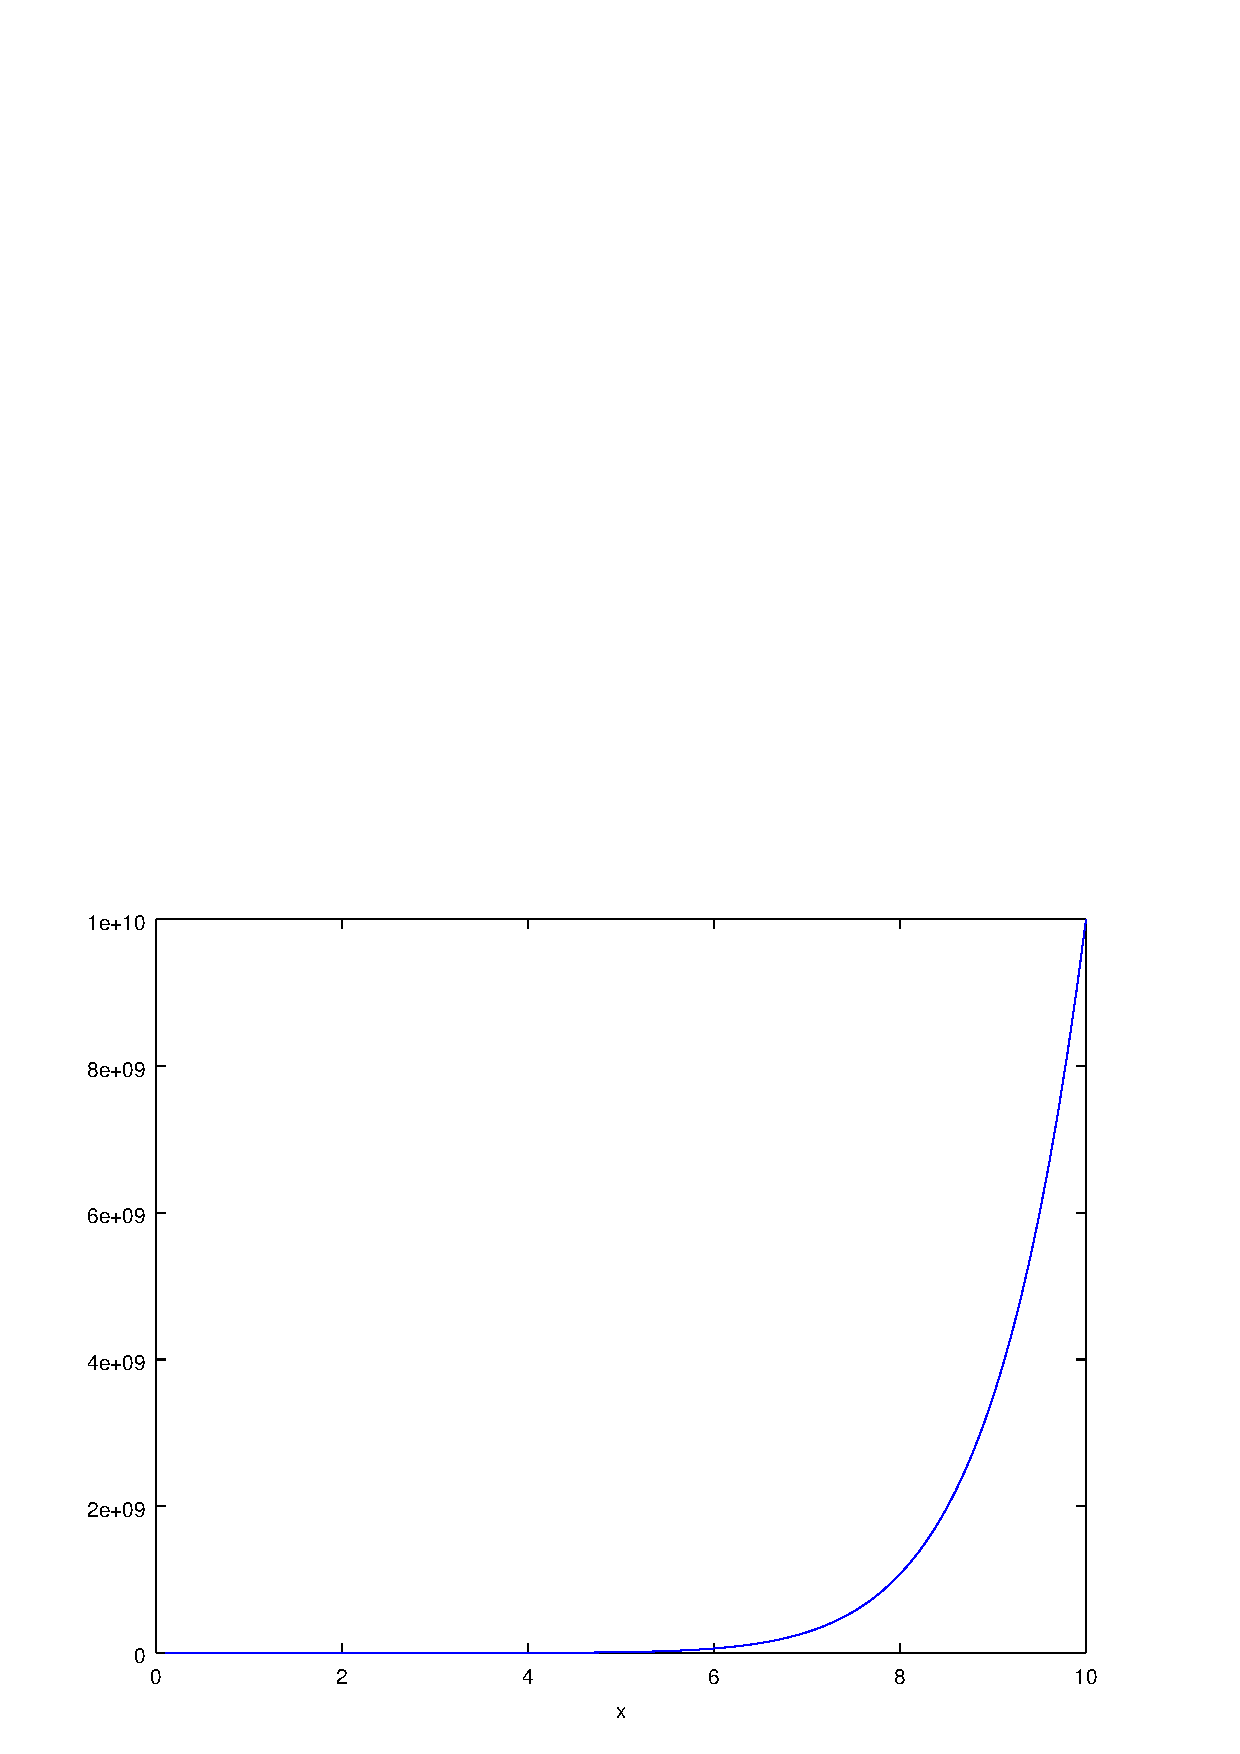
\includegraphics[width=0.5\textwidth]{1.png}
$\dfrac{dm}{dt}=\rho A \dfrac{dh}{dt}=q_{mi}-q_{mo}$
\begin{gather*}
\displaystyle
q_{mo} = q_{mi} - \rho A \frac{dh}{dt}=\frac{1}{R}P = \frac{\rho h(t)}{R}\\
q_{mi}-\rho A \frac{dh(t)}{dt} = \frac{\rho h(t)}{R}\\
\frac{1}{A}(\frac{q_{mi}}{\rho} - \frac{h(t)}{R}) =  \frac{dh(t)}{dt} =
\frac{h(t+\Delta t)-h(t)}{\Delta t} \\
h(t + \Delta t) = \frac{\Delta t}{A}(\frac{q_{mi}}{\rho} - \frac{h(t)}{R}) + h(t)\\
h(k+1) = \frac{\Delta t}{A}(\frac{q_{mi}}{\rho} - \frac{h(k)}{R}) + h(k)\\
\end{gather*}

\subsection{Find a DE for the following circuits.}
\subsubsection{}
\begin{gather*}
\displaystyle
Q = CV\\
V= \frac{Q}{C}\\
V(t) = \frac{1}{C}\int_{t_0}^{t} I(t) + V(t_0)\\
\because Q = \int_{t_0}^t I(t)\\
V = L\frac{dI(t)}{dt}\\
C\frac{dV(t)}{dt} = I(t) 
\end{gather*}

	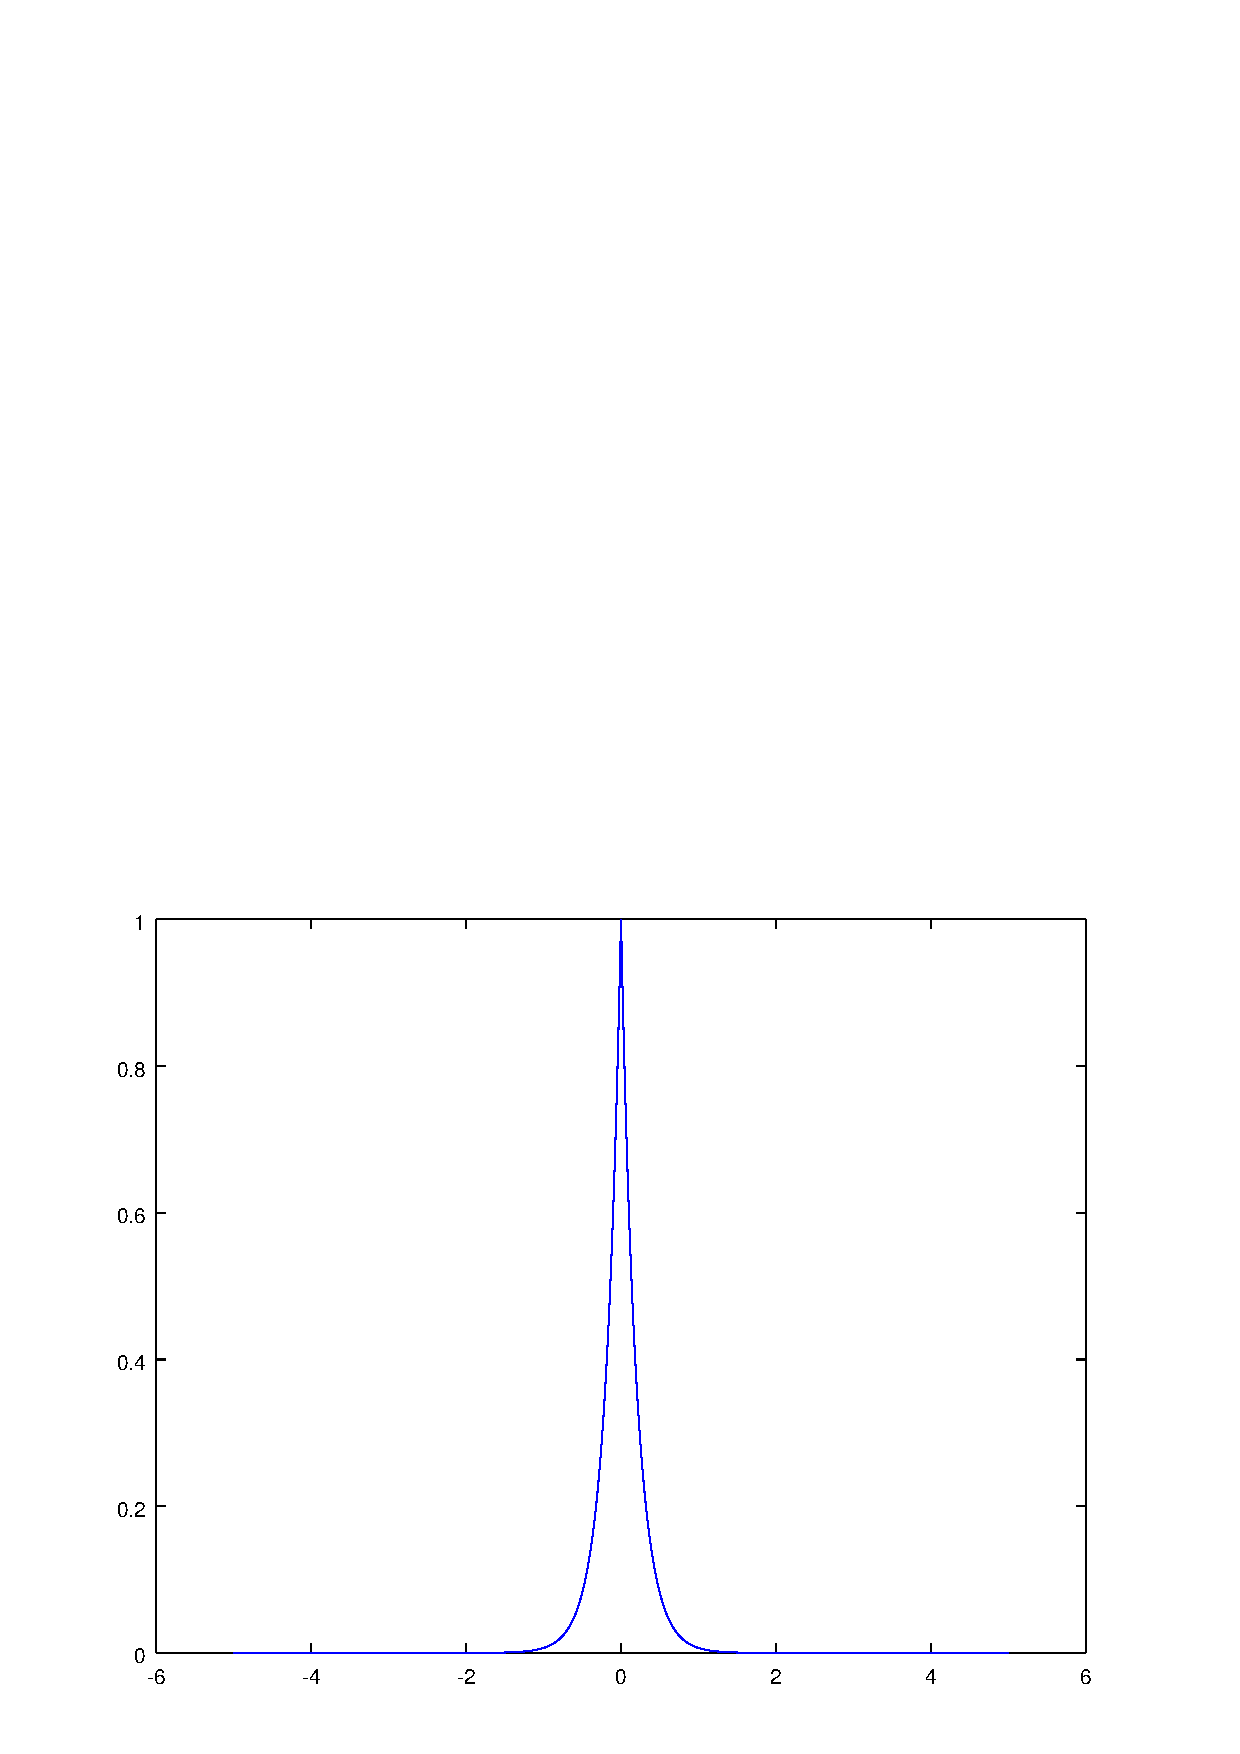
\includegraphics[width=\textwidth]{2.png}
	
	
\subsubsection{}
	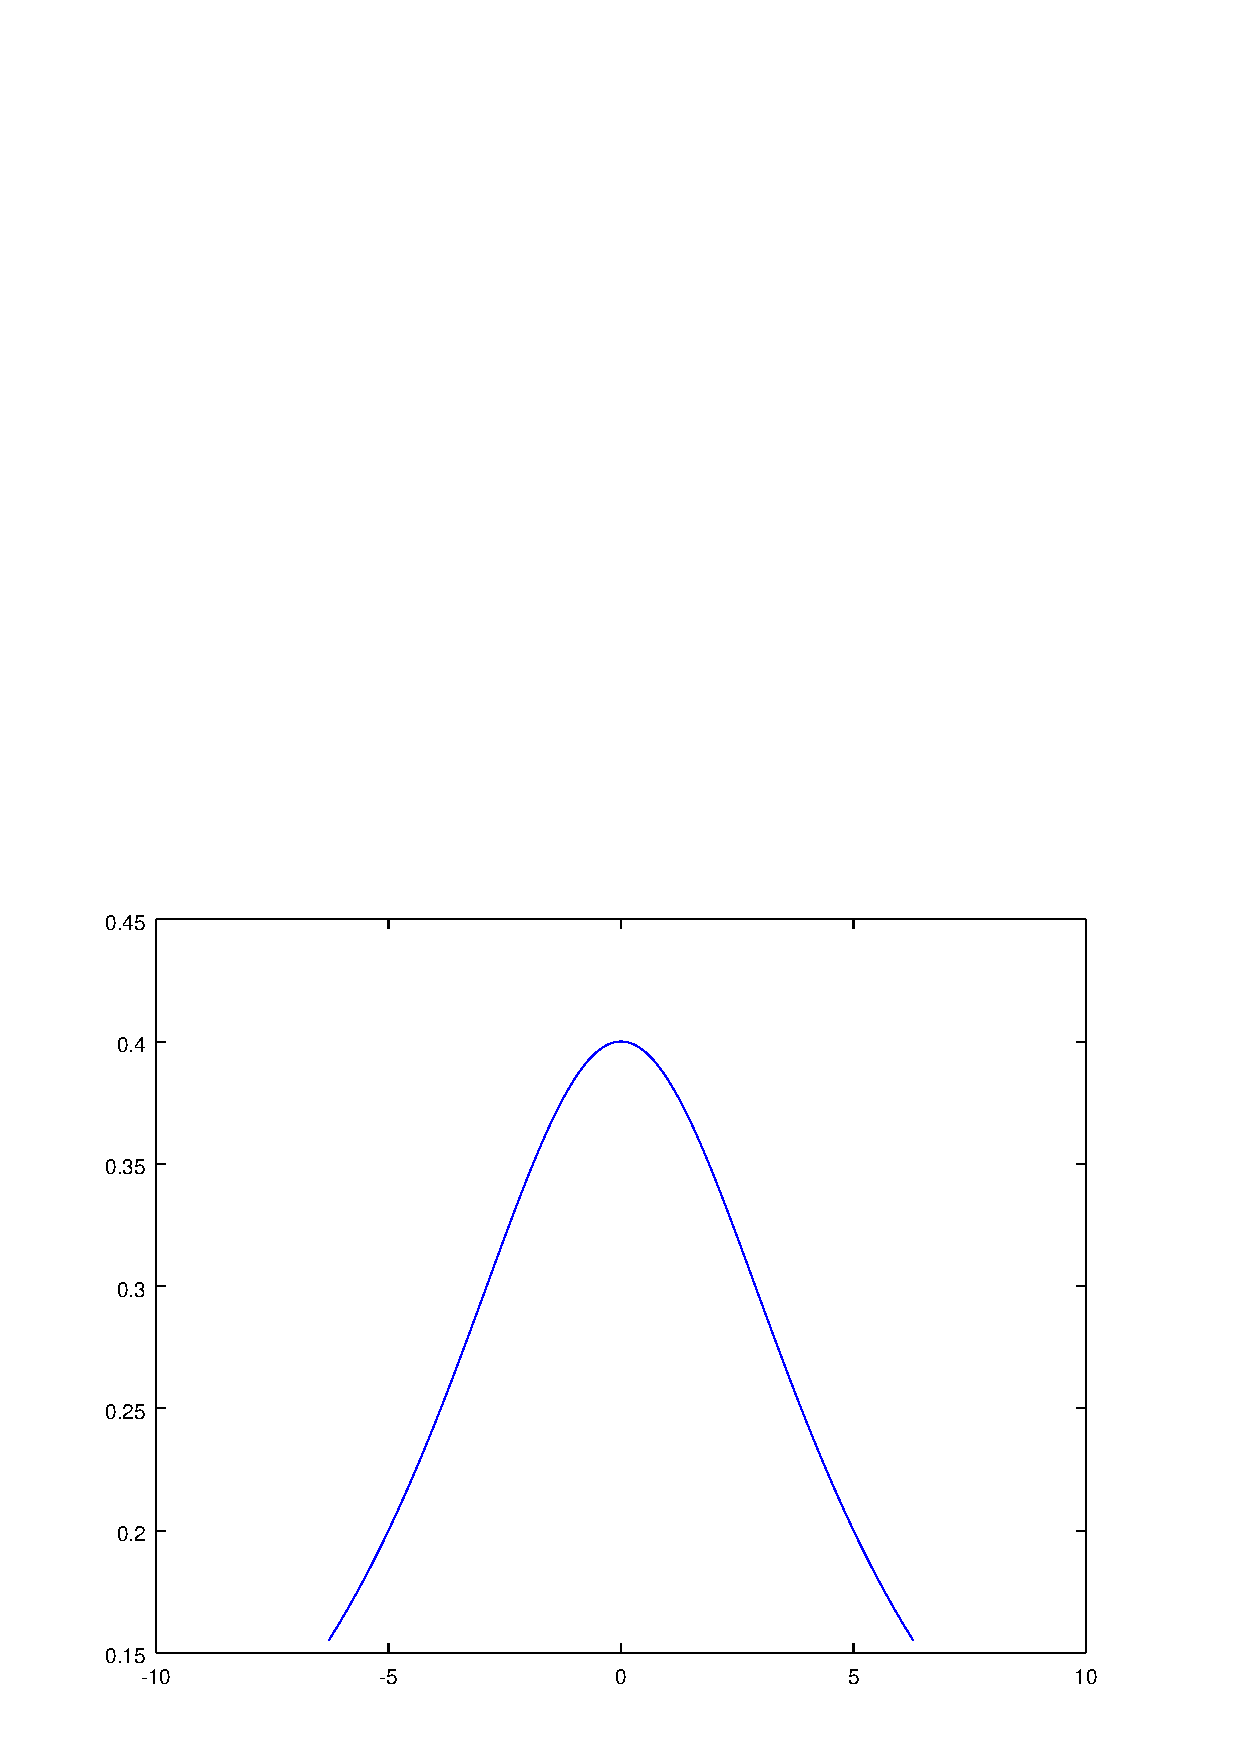
\includegraphics[width=\textwidth]{3.png}	
	
	
	
	
	
	

\end{document}
